\documentclass[11pt]{beamer}
\usepackage[utf8]{inputenc}
\usepackage{tikz}
\usepackage[T1]{fontenc}
\usetheme{Pittsburgh}
\usepackage{amsmath,tikz}
\usetikzlibrary{positioning}
\usetikzlibrary{shapes.geometric}


\newcommand\irregularcircle[2]{% radius, irregularity
	\pgfextra {\pgfmathsetmacro\len{(#1)+rand*(#2)}}
	+(0:\len pt)
	\foreach \a in {10,20,...,350}{
		\pgfextra {\pgfmathsetmacro\len{(#1)+rand*(#2)}}
		-- +(\a:\len pt)
	} -- cycle
}

\begin{document}
	\author{Tyne Team: S. Bogomolov, A. Hekal, M. Mehrabadi, S. Soudjani and P. Stankaitis}
	\title{F1Tenth, ROS and IROS F1/10 Virtual Competition}
	\institute{School of Computing, Newcastle University}
	\setbeamercovered{transparent}
	\setbeamertemplate{navigation symbols}{}
	\begin{frame}[plain]
	\maketitle
\end{frame}

\frame{Introduction and Background}

\begin{frame}{ROS: Robot Operating System}
\begin{itemize}
	\item[--] Not an actual operating system!
\end{itemize}
\end{frame}

\frame{IROS 2020 F1/10 Virtual Competition}

\begin{frame}{Tyne Team: Planning Algorithm}
\centering
\begin{figure}
	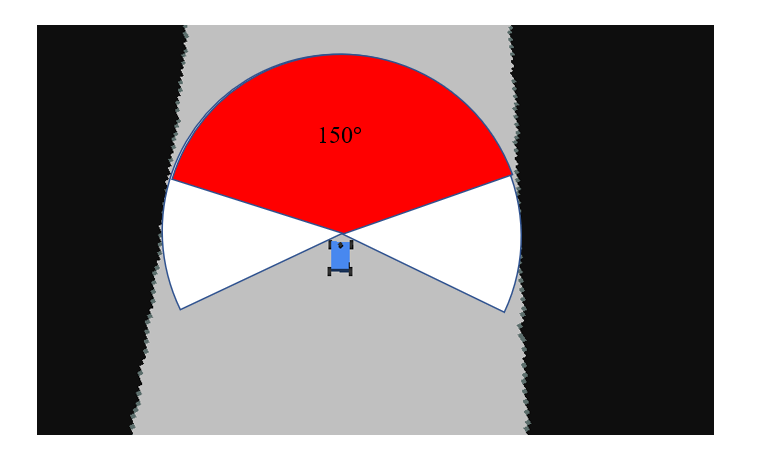
\includegraphics[scale=.4]{img/image1.png}
\end{figure}
\end{frame}

\begin{frame}{Tyne Team: Planning Algorithm}
\begin{figure}
	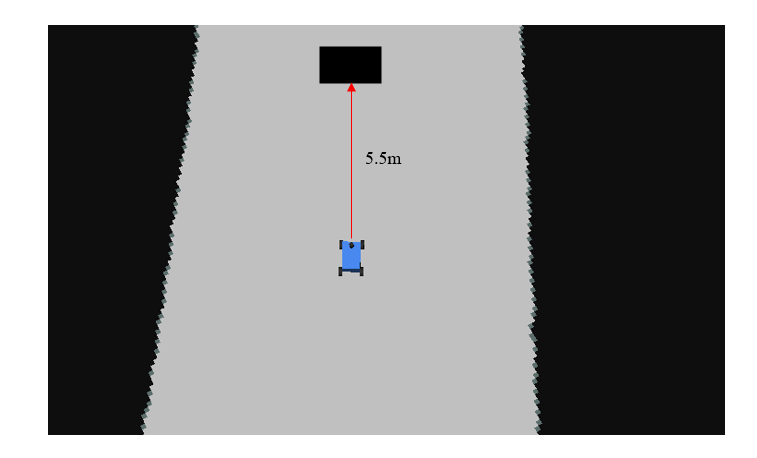
\includegraphics[scale=.4]{img/image2.png}
\end{figure}
\end{frame}

\begin{frame}{Tyne Team: Planning Algorithm}
$$Gap \; choice \; : \; \frac{\sum lidar_d - k * dev}{x^{0.3}}$$
\end{frame}



\begin{frame}{Tyne Team: Results}
\end{frame}

\begin{frame}{Tyne Team: Future Objectives}
\end{frame}

\end{document}

